\documentclass[12pt]{exam}
\usepackage[utf8]{inputenc}

\usepackage[margin=1in]{geometry}
\usepackage{multicol}
\usepackage{enumitem}
\usepackage{amsmath, amscd, amssymb, amsthm, xspace, graphicx}
%\usepackage{hyperref}
\usepackage[margin=1in]{geometry} % We can control the margins here
\usepackage[all]{xy}
\usepackage{subcaption}
\usepackage{float}
\usepackage{mathtools} 
%\usepackage{mcode}
\usepackage{listings}

\DeclarePairedDelimiter\Floor\lfloor\rfloor
\DeclarePairedDelimiter\Ceil\lceil\rceil

\newcommand{\class}{APPM 5600}
\newcommand{\term}{Fall 2023}
\newcommand{\examnum}{HW 1}
\newcommand{\mbbE}{\mathbb{E}}
\newcommand{\av}{\vec{a}}
\newcommand{\diffd}{\textnormal{d}}

%\numberwithin{equation}{section}
%\numberwithin{figure}{section}
%\numberwithin{table}{section}

\pagestyle{head}
\firstpageheader{}{}{}
\runningheader{\class}{\examnum\ - Page \thepage\ of \numpages}
\runningheadrule


\begin{document}

\noindent
\begin{tabular*}{\textwidth}{l @{\extracolsep{\fill}} r @{\extracolsep{6pt}} l}
	\textbf{Matthew LeDuc}&&\\
	\textbf{\class}&&\\
	\textbf{\term} &&\\
	\textbf{\examnum} &&\\
\end{tabular*}\\
\noindent

\section*{Question 1}
\subsection*{Part i}
I would multiply the function $f(x)=\sqrt{x+1}-1$ by the factor $\frac{\sqrt{x+1}+1}{\sqrt{x+1}+1}$. The function then is represented as 

\begin{equation}
f(x)=\frac{x}{\sqrt{x+1}+1}
\end{equation}
which is more numerically stable as it is not subtracting numbers that are potentially within $\epsilon_M$ of each other. 
\subsection*{Part ii}
We can apply the trigonometric identity

\begin{equation}
2\cos(\alpha)\sin(\beta) = \sin(\alpha+\beta)-\sin(\alpha - \beta)
\end{equation}

Letting $\alpha = \frac{x+y}{2}$ and $\beta=\frac{x-y}{2}$ we have that $\alpha+\beta=x$ and $\alpha-\beta=y$. Using this and the trigonometric identity, we can rewrite the expression as

\begin{equation}
\sin(x)-\sin(y) = 2\cos\left(  \frac{x+y}{2}\right)\sin\left(\frac{x-y}{2}\right)
\end{equation}

This expression is more stable since $\frac{1}{2}(\sin(x)-\sin(y) \le \frac{x-y}{2}$. This inequality can save us from potential subtraction issues when $x$ and $y$ are close but their difference is greater than $\epsilon_M$, while the different between their sines can possibly be less than $\epsilon_M$. 
\subsection*{Part iii}

We have two issues here: The first is that $1\approx \cos(x)$ and that $\sin(x)\approx x \approx 0$. We can remove both of these issues as follows:

First, note that
\begin{equation}
1-\cos(x) = \cos(0)-cos(x)=\cos\left(\frac{x}{2}-\frac{x}{2}\right)-\cos\left(\frac{x}{2}+\frac{x}{2}\right)
\end{equation}
and then we can apply the product to sum identities to show that 

\begin{equation}
\frac{1-\cos(x)}{\sin(x)} = 2\frac{\sin\left(\frac{x}{2}\right)^2}{\sin(x)}
\end{equation}

Applying the double-angle formula to the denominator, we see that 

\begin{equation}
\frac{1-\cos(x)}{\sin(x)} = \frac{\sin\left(\frac{x}{2}\right)}{\cos\left(\frac{x}{2}\right)}
\end{equation}

This new expression is more numerically stable, since it avoids both the potential for an accidental division by zero, since $\cos(0)=1$, and the subtraction of two numbers potentially within $\epsilon_M$ of each other. 
\newpage

\section*{Question 2}

\subsection*{Part i}
The function evaluated in its expanded form is shown in Figure \ref{fig:expanded}
\begin{figure}[h!]
\centering
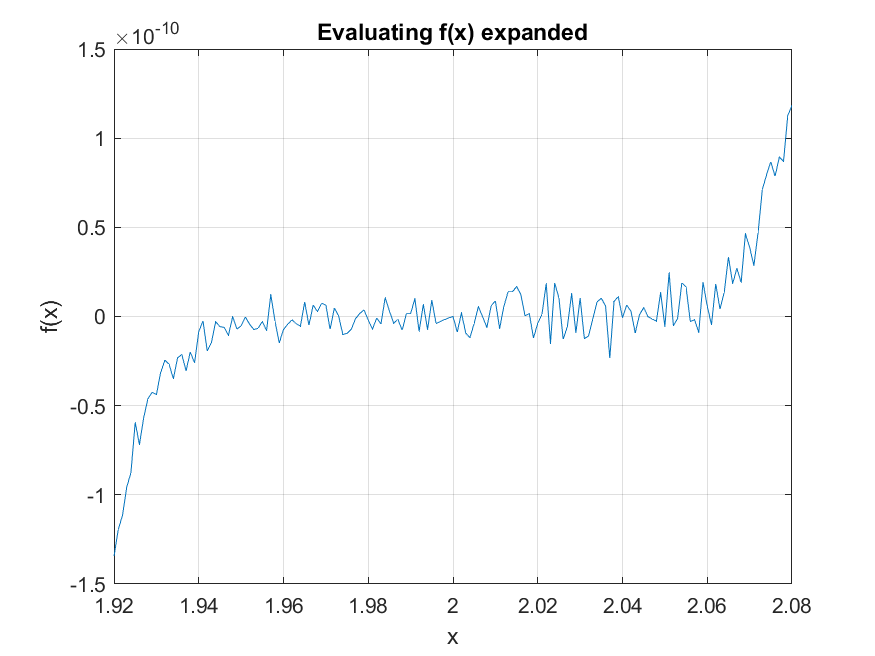
\includegraphics[width=0.5\textwidth]{q2p1.png}
\caption{p(x) evaluated in its expanded form}\label{fig:expanded}
\end{figure}
\subsection*{Part ii}
The function evaluated in its factored form is given in Figure \ref{fig:factored}
\begin{figure}[h!]
\centering
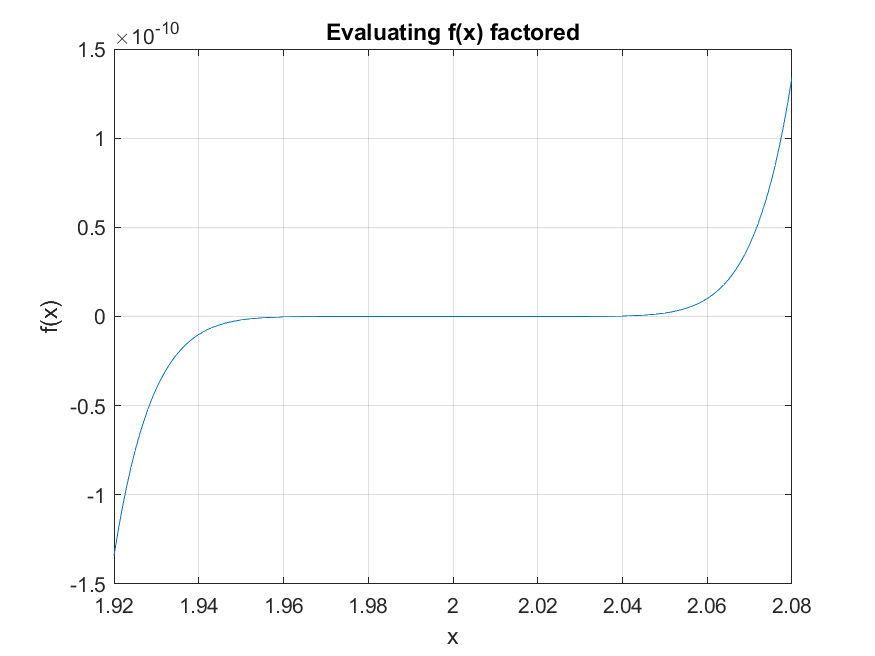
\includegraphics[width=0.5\textwidth]{q2p2.png}
\caption{p(x) evaluated in its factored form}\label{fig:factored}
\end{figure}
\subsection*{Part iii}

In Figure \ref{fig:expanded} the plot is not smooth at all. It appears that the function jumps randomly at each point. However, in Figure \ref{fig:factored} the plot is perfectly smooth. The second plot is correct, and the reason for the discrepancy is that since the values of $p(x)$ are so small, when evaluating each term individually the truncation errors at each point add up and cause relatively large discrepancies in the evaluation of the function, however when the function is evaluated in its factored form this does not occur.

\newpage

\section*{Question 3}

\subsection*{Part i}

\subsection*{Part ii}
We  can rewrite $f(x)$ as

\begin{equation}
\cos(x+\delta)-\cos(x)=\cos \left( \left(x+\frac{1}{2}\delta \right)+\frac{1}{2}\delta\right)-\cos\left(\left(x+\frac{1}{2}\delta\right)-\frac{1}{2}\delta\right)
\end{equation}
Then, using the fact that
\begin{equation}
2\sin(x)\sin(y)=\cos(x-y)-\cos(x+y)
\end{equation} 
the expression can be rewritten as 
\begin{equation}
f_2(x)=-2\sin\left( x+\frac{1}{2}\delta \right)\sin \left(\frac{1}{2}\delta\right)
\end{equation}

The difference between $f(x)$ and $f_2(x)$ is shown for $x=0,\frac{\pi}{3}, \frac{\pi}{4}, \frac{\pi}{2}$ and $\delta = 10^{-15}, 10^{-14},...,$ $10^{-1}, 1$ in Figure \ref{fig:fminusf2}.

\begin{figure}[h!]
\centering
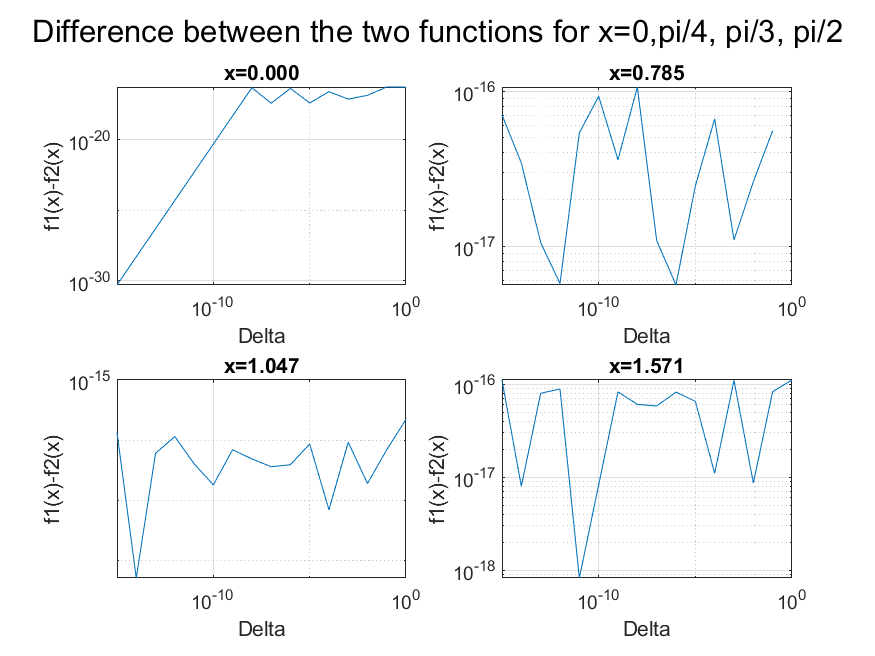
\includegraphics[width=0.5\textwidth]{q3p2.png}
\caption{Difference between $f(x)$ and $f_2(x)$ for various $x,\delta$}\label{fig:fminusf2}
\end{figure}
The difference tends to be on the order of $\pm 10^{-16}$ across all queried values of $x$ and $\delta$. 

\subsection*{Part iii}

The difference between $f(x)$ and the Taylor expansion is shown in Figure \ref{fig:fminusTaylor} for the same values of $x$ and $\delta$ as above. 
\begin{figure}[h!]
\centering
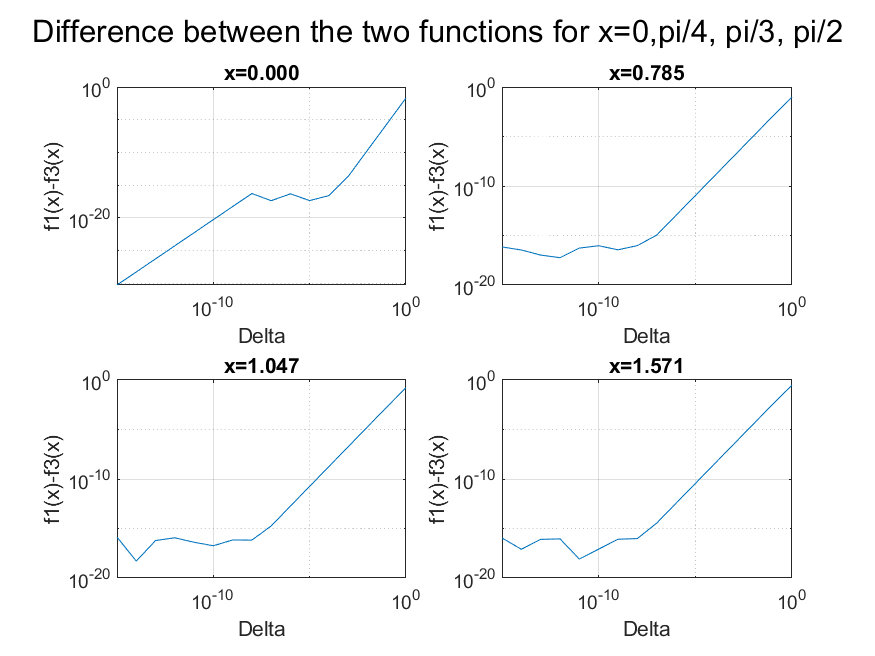
\includegraphics[width=0.5\textwidth]{q3p3.png}
\caption{Difference between $f(x)$ and the Taylor expansion for various $x,\delta$}\label{fig:fminusTaylor}
\end{figure}

From this figure, it appears that for each value of $x$, the Taylor expansion is closer to $f(x)$ than $f_2(x)$ for $\delta <10^{-10}$. Notably, the approximation gets much worse as $\delta$ increases, with the difference growing approximately linearly in $\delta$ for $\delta > 10^{-5}$. So, while this expression works well for smaller values of $\delta$ the error grows quickly as $\delta$ increases.
\subsection*{Code}
%\lstinputlisting{HW1_prob3.m}

\newpage

\section*{Question 4}

We say that $f(x)\sim o(g(x))$ as $x\rightarrow a$ if $\lim_{x\rightarrow a} \frac{f(x)}{g(x)}=0$. Now for any $n\in \mathbb{Z}$ let $f_n(x)=(1+x)^n$, and let $g(x)=x$. We divide the problem into cases.

 First consider the case $n=0$: Then $f(x) = 1+0x+0$ and since $\frac{0}{x}=0\ \forall x \ne 0$, we have that $\lim_{x\rightarrow 0} \frac{1-(1+0x)}{x}=0$ so $f_0(x)\sim 1+0x+o(x)$.

Now if $n=1,\ f(x)=1+x$ so again since $\frac{0}{x}=0\ \forall x \ne 0$, we have that $\lim_{x\rightarrow 0} \frac{1+x-(1+x)}{x}=0$ so $f_1(x)\sim 1+x+o(x)$.

Now let $n>1$. By the binomial theorem we can write that 

\begin{equation}
f_n(x) = \sum_{k=0}^n {n\choose k} x^k = 1+nx+x^2 \sum_{k=2}^n {n\choose k} x^{k-2} 
\end{equation}
and so given this, we wish to find the behavior of $x^2\sum_{k=2}{n}{n\choose k}x^{k-2}$ as $x\rightarrow 0$. Since

\begin{equation}
\lim_{x\rightarrow 0}\frac{1}{x} \left(x^2\sum_{k=2}^{n}{n\choose k}x^{k-2}\right) =  \lim_{x\rightarrow 0} x\sum_{k=2}^{n}{n\choose k}x^{k-2} =0 
\end{equation}
we have that $\lim_{x\rightarrow 0} \frac{f_n(x)-(1+nx)}{x}\sim o(x)$ as $x\rightarrow 0$, so $f_n(x) \sim 1+nx+o(x)$.

Lastly, let $n<0$. We can expand $f_n(x)$ in a Taylor Series as

\begin{equation}
f_n(x) = \sum_{k=0}^{\infty} \left[\frac{\diffd^k}{\diffd^k x}f_n(0)\right] \frac{x^k}{k!}
\end{equation}
Since $\frac{\diffd}{\diffd x} f_n(x) = n(1+x)^{n-1}$, we have that 

\begin{equation}
f_n(x) = 1+nx+x^2\sum_{k=2}^{\infty} \left[\frac{\diffd^k}{\diffd^k x}f_n(0)\right] \frac{x^{k-2}}{k!}
\end{equation}
and so we can write that 

\begin{equation}
\lim_{x\rightarrow 0}\frac{1}{x} \left(x^2\sum_{k=2}^{\infty} \left[\frac{\diffd^k}{\diffd^k x}f_n(0)\right] \frac{x^{k-2}}{k!}\right) =
  \lim_{x\rightarrow 0} x\sum_{k=2}^{\infty} \left[\frac{\diffd^k}{\diffd^k x}f_n(0)\right] \frac{x^{k-2}}{k!}=0 
\end{equation}
Therefore, we have that $\lim_{x\rightarrow 0} \frac{f_n(x)-(1+nx)}{x}\sim o(x)$ as $x\rightarrow 0$, so $f_n(x) \sim 1+nx+o(x)$.

The statement has been proven for all integers $n$, thus we have that $\forall n \in \mathbb{Z}$, $f_n(x) \sim 1+nx+o(x)$ as desired.
\newpage 

\section*{Question 5}

We say that $f(x) \sim O( g(x) )$ as $x\rightarrow a$  if $\limsup_{x\rightarrow a}\frac{|f(x)|}{g(x)} < \infty$. Letting $f(x)=x\sin(\sqrt{x})$ and $g(x) = x^{3/2}$, and noting that for small enough $x, f(x) = |f(x)|$, we have that 

\begin{equation}
\frac{f(x)}{g(x)} = \frac{x\sin(\sqrt{x})}{x^{3/2}} = \frac{\sin(x^{1/2})}{x^{1/2}}
\end{equation}
and, by applying L'Hopital's rule, we have that 

\begin{equation}
\limsup_{x\rightarrow 0}  \frac{\sin(x^{1/2})}{x^{1/2}} = \lim_{x\rightarrow 0}  \frac{\sin(x^{1/2})}{x^{1/2}} = \lim_{x\rightarrow 0} \cos( \sqrt{x} ) = 1
\end{equation}

Therefore, since $\limsup_{x\rightarrow 0}\frac{x\sin(x^{1/2})}{x^{3/2}} < \infty$ we say that $x\sin(x^{1/2}) \sim O( x^{3/2} )$ as $x\rightarrow 0$.

\newpage 

\section*{Question 6}

\subsection*{Part i}
Using the factored form of the function, the bisection method converges to $x=5$ in $13$ iterations. 

\subsection*{Part ii}
Using the expanded form of the function, the bisection method converges to $x\approx 5.08149$ in $13$ iterations. 
\subsection*{Part iii}
The repeated truncation error from adding each term of the expanded form of the function leads to an error in the function evaluation, and this error changes where the algorithm will observe the root to be. Even though the actual root of the function is at $x=5$, these repeated truncation errors add up in such a way that the evaluation of the function finds a root in the wrong place. 
\subsection*{Code}
%\lstinputlisting{HW1_prob6.m}

%\newpage
%\section*{Appendix}




\end{document}